\chapter{Introduction}

\section{Installation}
Neverblender requires Blender 2.69 or newer. Neverblender can be installed
like every other add-on:
\begin{enumerate}
\item Open \menu{File > User Preferences} and under Add-ons, 
click \menu{Install from File...}. Then navigate to the file you downloaded and select it.
\item It will now appear in the window as \textit{Import-Export: Neverblender}. Tick the checkbox in the upper right to enable it.
\item To have the add-on enabled every time you start Blender, click \menu{Save User Settings} at the bottom.
\end{enumerate}
Manual installation is possible by extracting the contents of the downloaded archive and 
placing the \directory{neverblender} folder in Blender's \directory{scripts/addons} directory. 
It is recommended to also install the \href{https://wiki.blender.org/index.php/Extensions:2.6/Py/Scripts/Animation/AnimAll}{AnimAll}\footnote{\href{https://wiki.blender.org/index.php/Extensions:2.6/Py/Scripts/Animation/AnimAll}{https://wiki.blender.org/index.php/Extensions:2.6/Py/Scripts/Animation/AnimAll}} add-on, which will facilitate the 
editing of Animmeshes (= Meshes with animated texture coordinates). \textit{AnimAll} ships with 
blender, but is disabled by default. It is listed as \textit{Animation: AnimAll}.

\begin{figure}[hb]
    \centering
    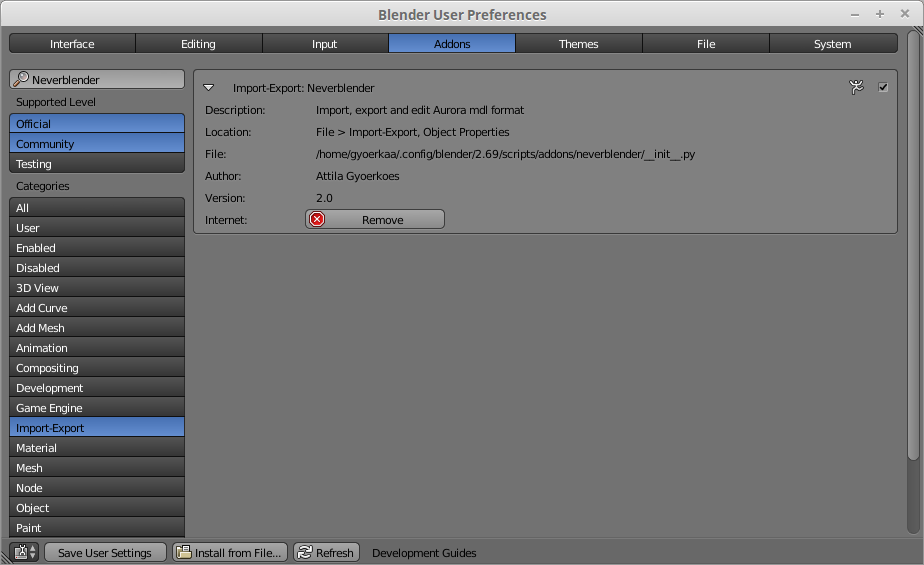
\includegraphics[width=\linewidth]{window_userprefs}
    %\caption[Close up of \species{Hemidactylus}]
    %{Close up of \species{Hemidactylus}, which is part the genus of the gecko family. It is the second most speciose genus in the family.}
\end{figure}

\section{User Interface}
Once installed, additional entries are available in Blender's menu: \menu{File > Import > Aurora (.mdl)} and 
\menu{File > Export > Aurora (.mdl)}. Furthermore several new panels are added to the Object Properties window:
\begin{itemize}
\item Aurora Root Properties: Shown whenever an object belonging to a MDL is selected.
\item Aurora Dummy Properties: Shown whenever an Empty with a parent is selected.
\item Aurora Mesh Properties: Shown whenever a Mesh is selected.
\item Aurora Animation Properties: Shown whenever an object belonging to a MDL is selected.
\item Aurora Utilities: Shown whenever an object belonging to a MDL is selected.
\end{itemize}